\documentclass[12pt]{article}
\usepackage[utf8]{inputenc}
\pagenumbering{arabic}
\usepackage{graphicx}
\usepackage{amstext}
\usepackage[usenames, dvipsnames]{color}
\usepackage{array}
\usepackage{float}
\usepackage{enumitem}
\usepackage[top=1.5in]{geometry}
\usepackage{subcaption}
\graphicspath{ {images/} }

\begin{document}

\begin{titlepage}
    \begin{center}
    \begin{figure}
        \centering
        
\includegraphics[scale=0.2]{logoPolimi.png}
        \vspace{1.5cm}
    \end{figure}

    \Huge\textbf{Software Engineering 2 Project - TrackMe}
    \rule{12cm}{0.5pt}
    \Huge\textbf{Requirement Analysis and Specification Document - V1}
    \today
    \end{center}
    
    \vspace{3cm}
    
    \begin{flushleft}
        \LARGE\textbf{Authors: }
        \newline\newline
        \Large\texttt{}{Michiel Janssen \\ Erbol Kasenov \\ Lorenzo Casalini}
    \end{flushleft}
\end{titlepage}

\newpage
  \tableofcontents
\newpage

\section{Introduction}
\subsection{Purpose}
This document represents the Requirement Analysis and Specification Document (RASD). Goals of this document are to completely describe the system in terms of functional and non-functional requirements, analyze the real needs of the customer in order to model the system, show the constraints and the limit of the software and indicate the typical use cases that will occur after the release. This document is addressed to the developers who have to implement the requirements and could be used as a contractual basis.
\subsection{Scope}
TrackMe is a company that wants to develop a software-based service allowing third parties to monitor the location and health status of individuals. The main service, Data4Help, supports the registration of individuals (of any age) and third parties. Upon registration the individual agrees that TrackMe acquires their data. This data can be obtained from smartwatches or similar devices. After registration a third party can request the following things:
\begin{itemize}
\item Access the data of a specific individual by entering a unique number or code. TrackMe passes the request to the specific individual who can accept or refuse the data acquisition.
\item Access anonymized data of groups of individuals given by a specific constraint e.g.: every individual older than 30 years, every individual that is male or female, etc. These requests are handled and approved by TrackMe if and only if TrackMe can guarantee that they are able to properly anonymize the requested data.
\end{itemize}
As soon as a data request is approved, TrackMe makes the previously saved data available to the third party. The service also allows a third party to subscribe to new data and listen to new data as soon as they are produced. With the data acquired through Data4Help, it will be also possible to offer two other services based on the retrieved data. The first service is a personalized and non-intrusive SOS service, called AutomatedSOS, to help elderly people. This service monitors the health status of subscribed customers and sends an ambulance to this specific customer if some parameters are below a certain threshold. The reaction time should be less than 5 seconds from the time the parameters are below the certain threshold.
The second service, called Track4Run, allows organizers to define a path for a run, participants to enroll to a certain run and spectators to see the position of all current running participants on a map.

\subsection{Definitions, Acronyms, Abbreviations}
\subsubsection{Definitions}
\begin{itemize}
\item \textit{Visitor}: A person who uses TrackMe for the first time, and is not yet registered. This can be an individual or a third party. After a successful registration process the person becomes an individual and is now able to use TrackMe services.
\item \textit{Individual}: A registered person who uses TrackMe for monitoring his location and health status.
\item \textit{Third party}: A registered organization that wants to access the location and health status of specific individual by giving a social security number of that individual.
\item \textit{Home Screen}: User interface screen that shows the current appointments.

\item \textit{System}: defines the overall set of software components that implement the required functionality.
\end{itemize}


\subsubsection{Acronyms}
\textit{API}: Application Programming Interface\newline
\textit{RASD}: Requirements Analysis and Specification Document\newline
\textit{SQL}: Structured Query Language\newline
\subsubsection{Abbreviations}
\textit{Gn}: Goal defined with index n.\newline
\textit{Dn}: Domain Assumption defined with index n.\newline
\textit{Rn}: Functional Requirement defined with index n.
\subsection{Revision History}
\subsection{Reference Documents}
\begin{itemize}
\item Assignment document: Mandatory Project Assignment AY 2018-2019.pdf
\item IEEE Recommended Practice for Software Requirements Specifica- tions (Std 830-1998)
\end{itemize}
\subsection{Document Structure}
Other than this introductory chapter, this RASD is organized in six more chapters. Chapter two is meant to provide an overview of the system’s functionality, the type of users it is meant for and the different kinds of interactions it contemplates, not only with the users themselves but also with other systems. Some of the systems require- ments are also slightly discussed in this chapter, even though they’ll be analyzed in the following chapter. In the third chapter (as mentioned) the system requirements, attributes and constraints are analyzed and discussed in the appropriate detail and depth, specifying exactly how they should be. The fourth chapter deals with the for- mal analysis of the system using an Alloy model. It includes the Alloy model of the system with a brief discussion on its purpose and on the relevance of using Alloy as a tool to validate our solution, given the problem we had to solve. In the fifth chapter the effort spent by each of the group members is described by specifying the number of hours each member of the group worked on the development of this document, and on the final chapter the tools we used to develop this RASD are specified.

\section{Overall Description}

\subsection{Product Perspective}
In general the system will need to communicate with several existing systems through an API. At first we need to have devices that track specific paramaters for an individual. This can be done with the following possible devices (not all possible devices are given but the most important one's): 
\begin{itemize}
    \item Smartwatch: measure heart rate, distance traveled, calories burned, ...
    \item Blood sugar control device: measure glucose level in the blood
    \item Smartphone: distance traveled, step tracking, floors climbed, ...
    \item Thermometer: measure the temperature of an individual
\end{itemize}
All these devices, if ever used, must properly cooperate with our system in order to monitor the health status of the individual. Moreover the system needs to communicate with the Google Maps API in order to track the current location of an inidividual.
The description above describes what is needed for Data4Help service. In addition their are two other services called AutomatedSOS and Track4Run build on top of Data4Help. For the first service, the system needs to communicate with an ambulance system in Milan in order to send an ambulance on time when an individual (in danger) is required to have one. For the second service no other external service is needed. It will just exploit the features offered by Data4Help.
\subsection{Product Functions}
Considering all of the presented goals of the TrackMe system, the majority of functions of the system can be divided into 3 groups. In the following section, they are listed and more precisely specified, with respect to the already mentioned goals of the system.
\subsubsection{Data4Help}
The application gives you 2 types to login. The first way is the one to login as a user. The user can check his own location, track his motion path and time, and see health indicators. The second way is the one to login as a third party. A third party could check the location and health data of users by giving in an social security number (or something similar) of an individual. All these features combined form the Data4Help service.
\subsubsection{AutomatedSOS} This service also monitors the health parameters of subscribed individuals. When specific parameters are below a certain threshold it alarms an ambulance and the service passes them the location of the individual in danger. The service guarantees a reaction time less than 5 seconds from the time the parameters are below the threshold.
\subsubsection{Track4Run}
This service makes it possible for inidividuals to organize a certain path for a run comptetion. Individuals have also the possibility to join the run or track the location of all runners during the run. For monitoring the athletes who are participating in the run, the service exploits the features offered by Data4Help. 

\subsection{User Characteristics}
The system aims at satisfying the needs of two different types of users. The first type is the individual, the individual is the one who wants their health and location to be tracked and monitored. A lot of individuals will have several devices that track health data about them, this can be a smartphone, a smartwatch, etc. Therefore the purpose why individuals are using TrackMe, is that they need an application to improve the way their health data is being organized. They want to have one application where the data from all their devices is being displayed. The second type is the third party. A third party can be an organization like a hospital, a sporting company, etc. Their main purpose is that they need data to work with inside their organization. We assume that the individuals

\subsection{Assumptions, dependencies and constraints}
[D1] The username and email must be unique. \newline
[D2] The system will have access to the smartphone/smartwatch GPS functionality. \newline
[D3] The phone will always have a connection to the internet (WiFi or mobile data). \newline
[D4] Individuals are using a smartwatch and a smartphone to monitor the health status. They can have additional devices to monitor specific paramaters but this is not necessary.\newline
[D5] Individuals accept to share their data with the application's online database. \newline
[D6] The external services used by the system are assumed to be always available and reachable. \newline
[D7] The threshold of the health status parameters are fixed unless an individual/third party changes them. \newline
[D8] Data (health or location) maps only to one specific inidividual. \newline
[D9] The location of individuals is always known by the system. \newline
[D10] General info (length, weight, gender, date of birth, fiscal code) is given by the individual upon registration. \newline


\subsubsection{Hardware limitations}
\begin{itemize}
    \item Mobile application
    \begin{itemize}
        \item iOS or Android smartphone
        \item 2G/3G/4G connection
        \item GPS
    \end{itemize}
    \item Devices
    \begin{itemize}
        \item Smartphone
        \item Smartwatch
        \item Blood sugar control device
        \item Thermometer
        
    \end{itemize}
\end{itemize}

\section{Specific Requirements}

\subsection{External Interface Requirements}

\subsubsection{User Interfaces}
The following Mockups represent a basic idea of how the systems user interface will look like on the first release (mobile application):
\begin{itemize}
    \item Figure 1 and 2 show the login screen and registration screen for an individual and a third party.
    \item Figure 3 shows the different windows you have in the home screen. The first screen is today's activities, activities like for example walked and running distance are showed for a specific day. The second screen is health data where we can find detailed information about an individual such as hearthbeat, blood pressure, etc. In figure 4 (left) we find the third screen, the one who makes it possible to make/enroll/spectacte a run. These screens are only available for indivduals. The right screen in figure 4 is ment to be for third parties. They can enter a fiscal code of an individual they want to track and enter a data request as well. 
\end{itemize}

\newpage
\begin{figure}[t!]
\centering
    \begin{subfigure}{.4\textwidth}
        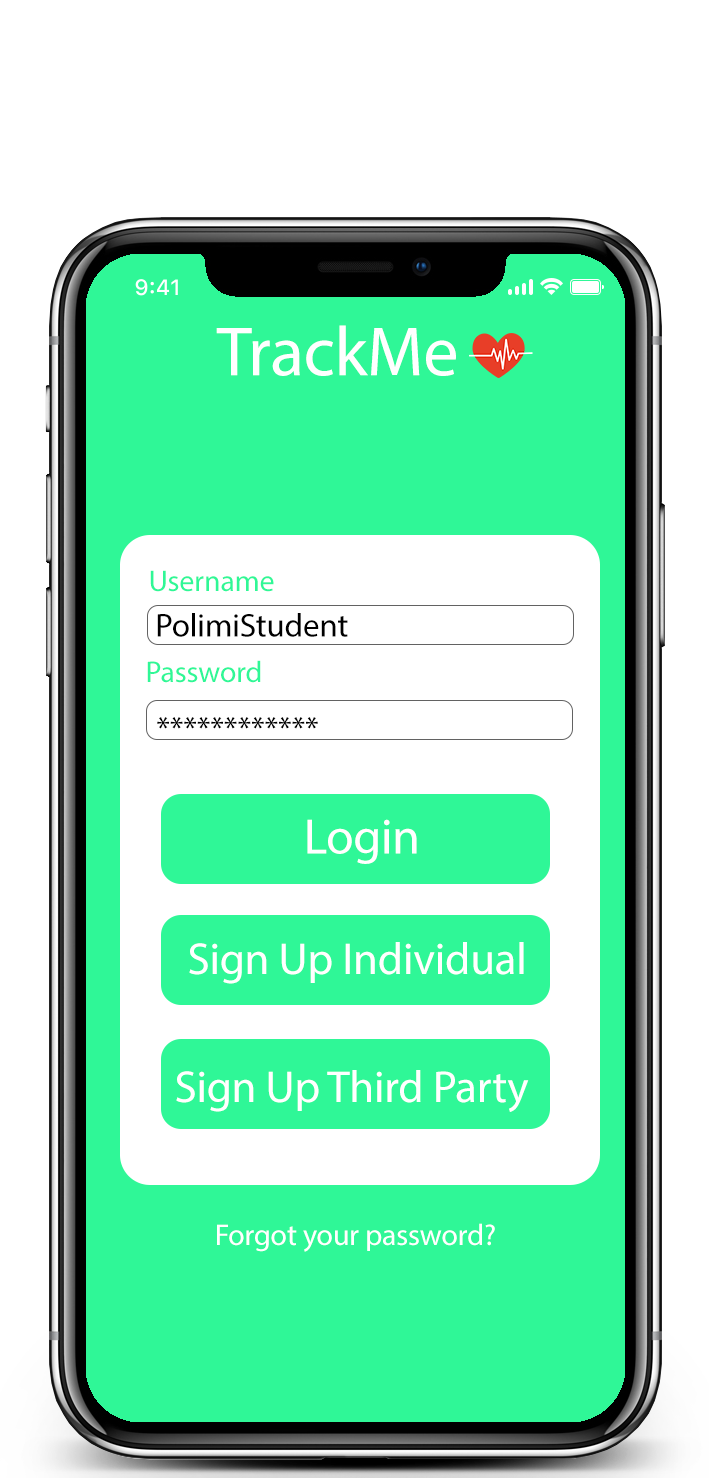
\includegraphics[scale=0.2]{LoginScreen.png}
        \label{fig:loginScreen}
    \end{subfigure}%
    \begin{subfigure}{.4\textwidth}
        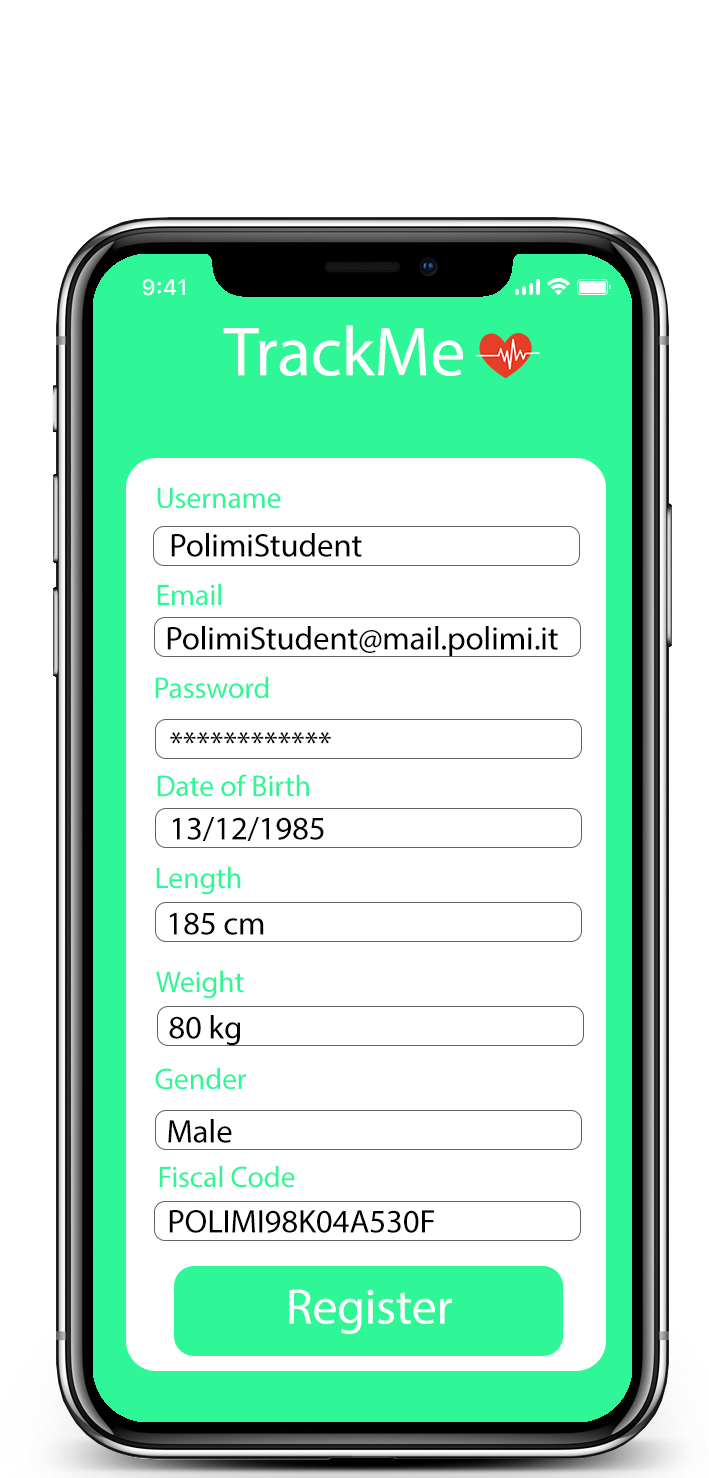
\includegraphics[scale=0.2]{RegisterScreen-Individual.png}
        \label{fig:RegisterScreen-Individual}
    \end{subfigure}
    \caption{Login Screen (left) and  Register Screen for an individual (right)}
\end{figure}

\begin{figure}[H]
\centering
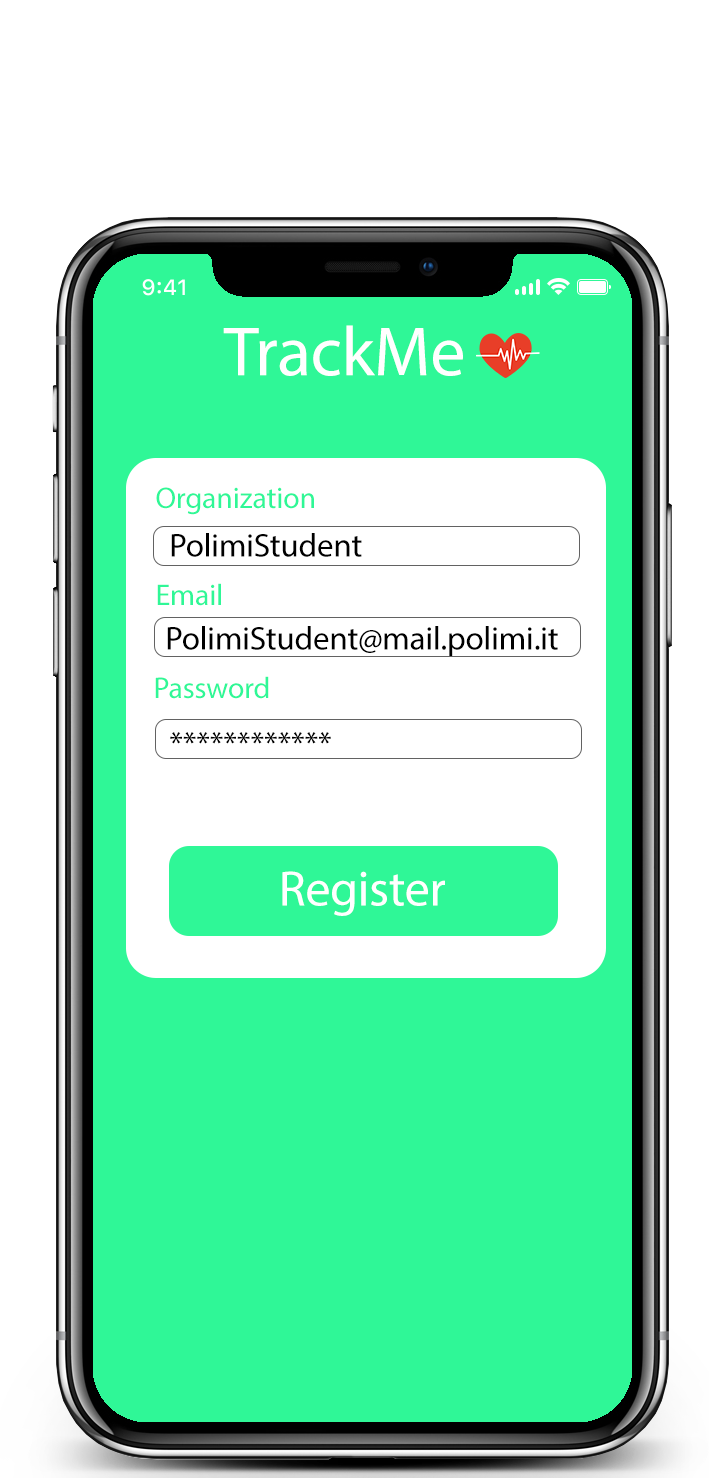
\includegraphics[scale=0.2]{RegisterScreen-ThirdParty.png}
\label{fig:RegisterScreen-ThirdParty}
\caption{Register Screen for a Third Party.}
\end{figure}

\begin{figure}[t!]
\centering
    \begin{subfigure}{.4\textwidth}
        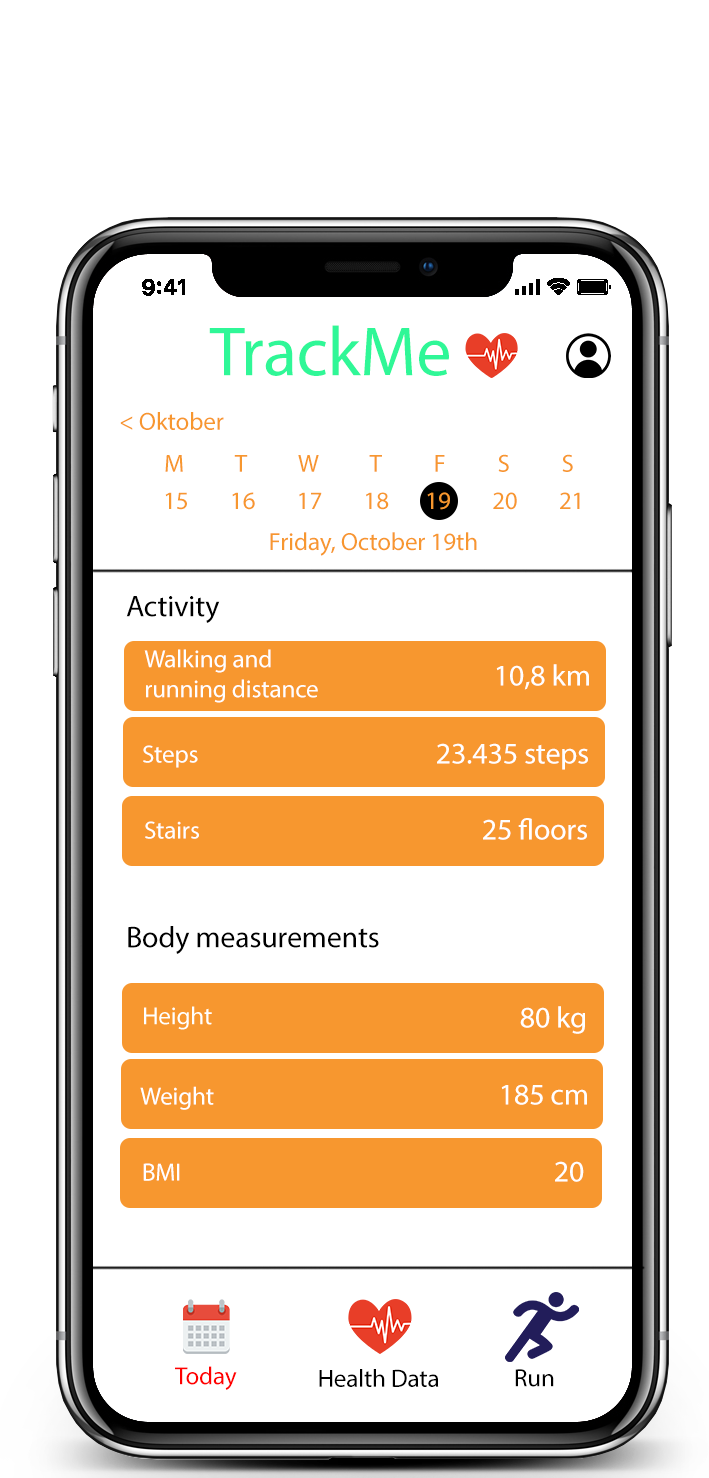
\includegraphics[scale=0.2]{HomeScreen1.png}
        \label{fig:HomeScreen1}
    \end{subfigure}%
    \begin{subfigure}{.4\textwidth}
        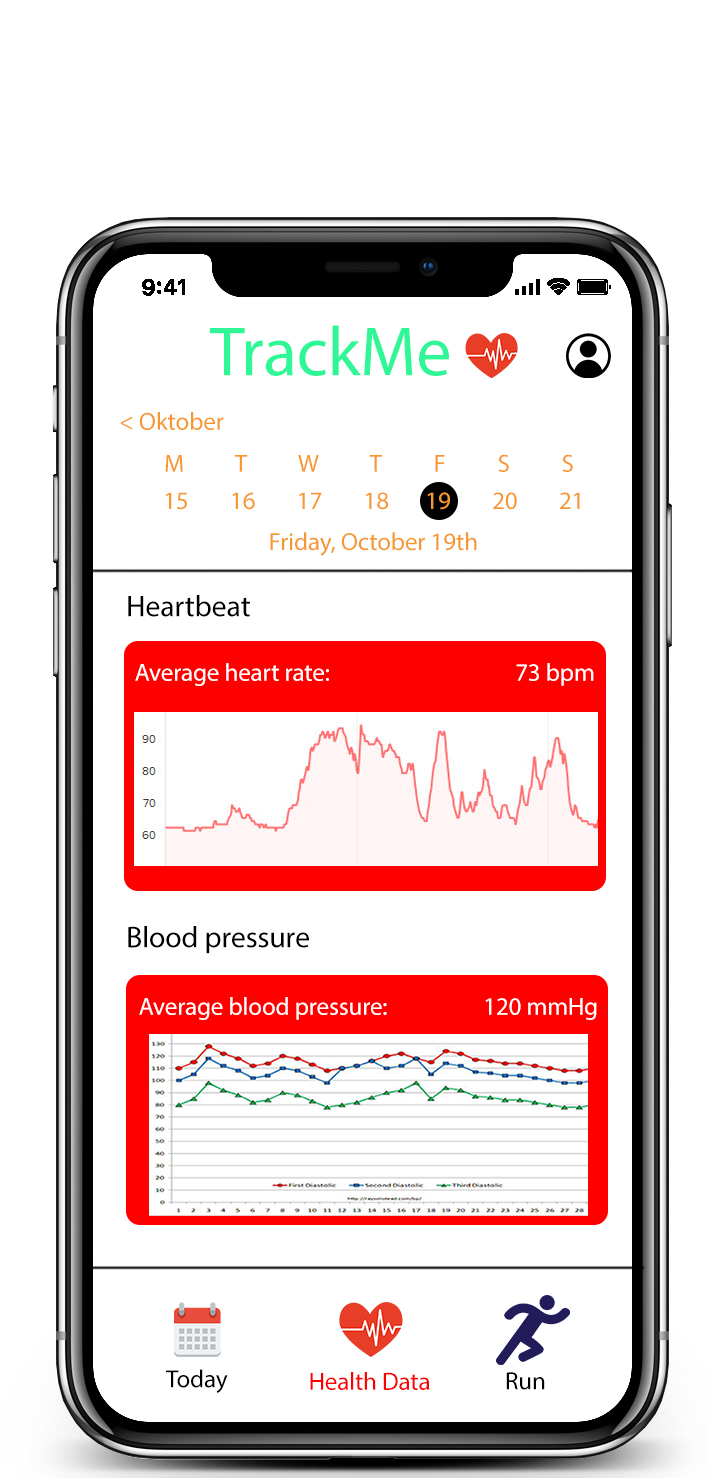
\includegraphics[scale=0.2]{HomeScreen2.png}
        \label{fig:HomeScreen2}
    \end{subfigure}
    \caption{Home Screen: Today's activities (left) and Health Data (right)}
\end{figure}

\begin{figure}[H]
\centering
    \begin{subfigure}{.4\textwidth}
        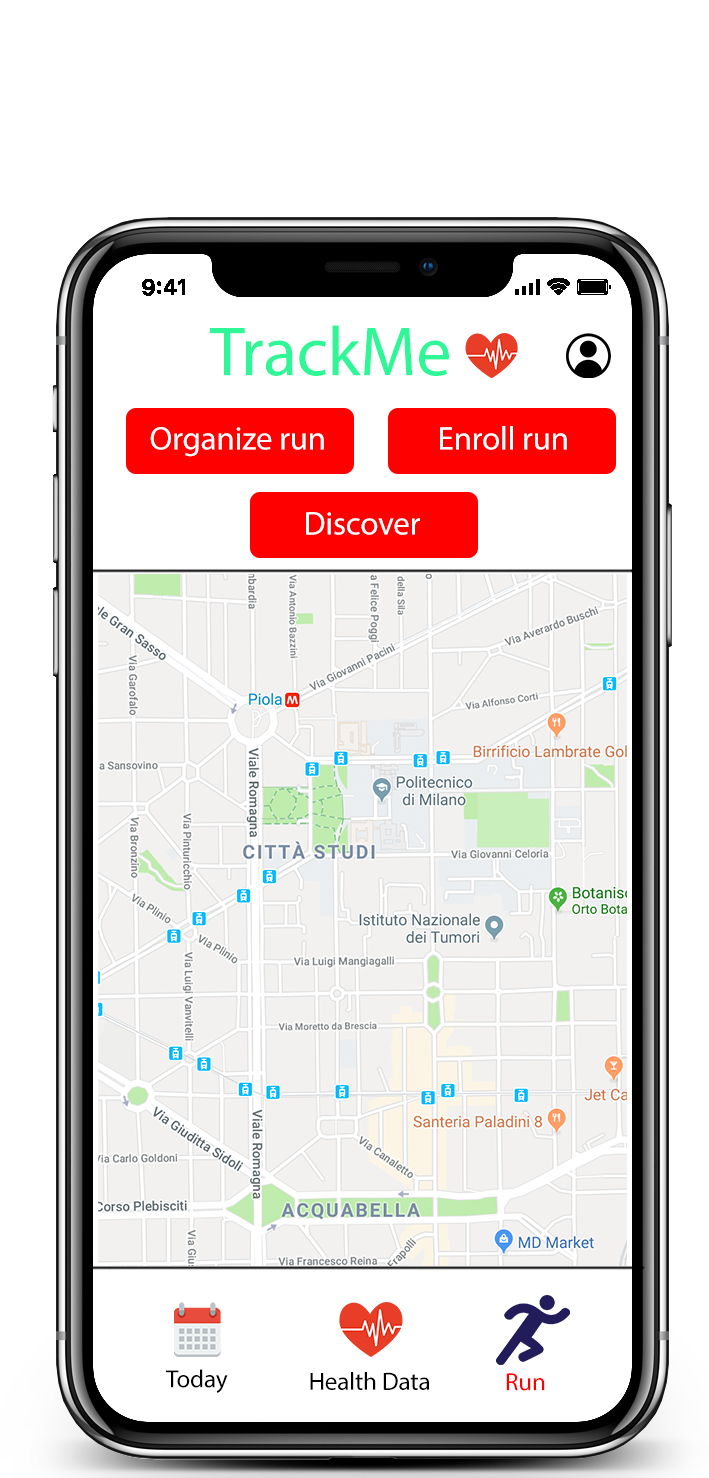
\includegraphics[scale=0.2]{HomeScreen3.png}
        \label{fig:HomeScreen1}
    \end{subfigure}%
    \begin{subfigure}{.4\textwidth}
        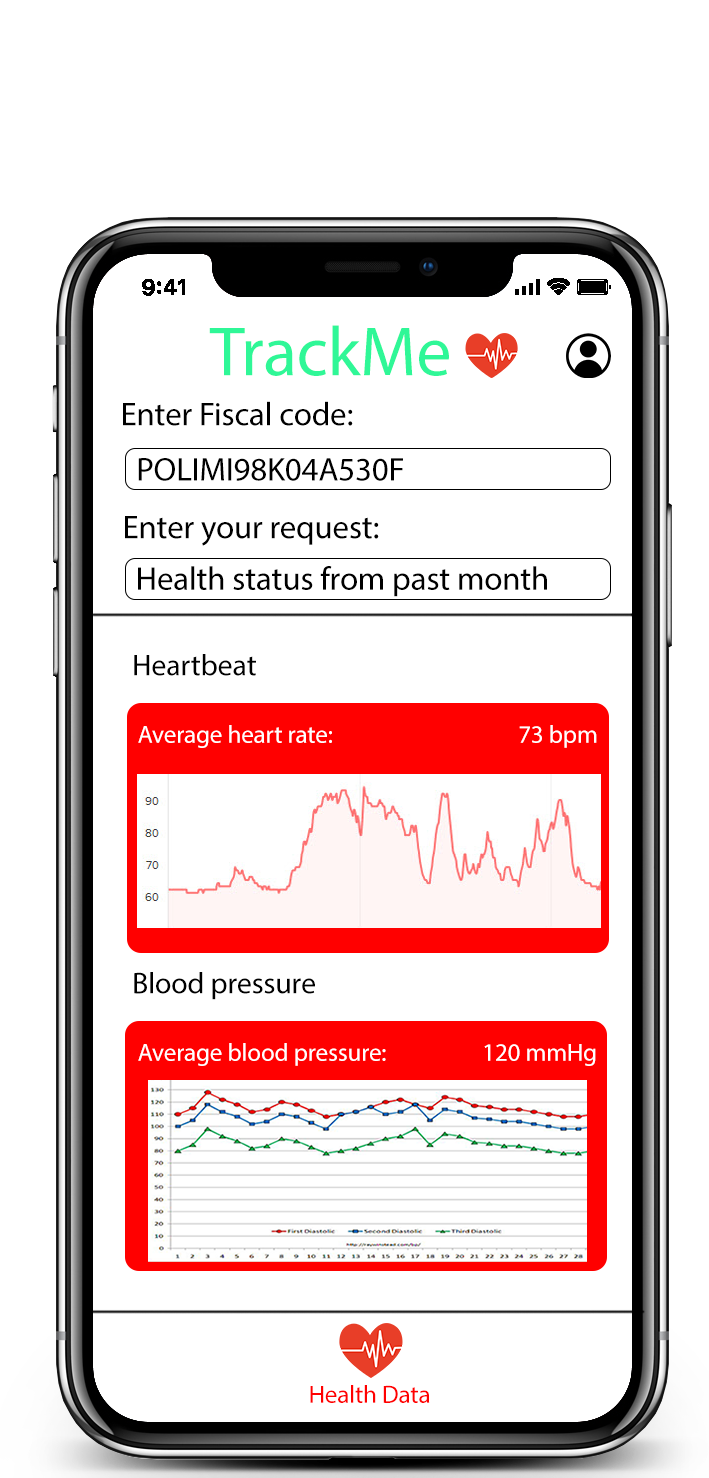
\includegraphics[scale=0.2]{HomeScreen4.png}
        \label{fig:HomeScreen2}
    \end{subfigure}
    \caption{Home Screen for individual (left) and for a third party (right)}
\end{figure}


\subsubsection{Hardware Interfaces}
In the first release, no Hardware Interfaces will be necessary since the system doesn’t need to interact physically with other systems.
\subsubsection{Software Interfaces}
Given the wide range of features the system offers, it will need to have several software interfaces. There has to be a way of storing all the user-related data (mainly login, general info, location and health data). In that sense, the system will use a \textbf{MySQL API} to connect with our MySQL database server, where all the application data will be stored. The system will also need different kinds of information about the individuals location, in order to combine health data with a location. To support this functionality, the system will use \textbf{Google Maps Geolocation API} and \textbf{Google Maps API}. The first one will provide information about the individual exact location and the second one will provide the real-time information about maps. The last will allow individuals to define a path for a run and for others to see the route for the run. To have access to the ambulance dispatch system and send them a request for an ambulance if an individual is in danger, our system will have an interface with \textbf{Ambulanza Milano}. At last, all the health data will come from several different devices and possibly from other brands as well. To gather all this health data we need to use serveral API's. Since a lot of devices (smartwatch, blood pressure device, ...) are seamlessly working with iOS and Android we need to communicate with iOS and Android API's. Considering a lot of third-party applications who offer a specific health tracking application, like measuring the blood control for a diabetic person, work with \textbf{HealthKit} and \textbf{Google Fit}, we will mainly use these two for keeping track of the health status of the individuals. 

\subsubsection{Communication Interfaces}
Communication interfaces ensure the communication between the system and the other software interfaces (third party service providers). The communication between the system and those service providers is crucial because the system depends on those services to perform its functions. Given this, the systems communication interface must be either WiFi or Mobile Data (2G, 3G or 4G), and the service providers communication interface can be of any type, as long as it ensures that they are connected to the internet. The protocol used shall be HTTPS, in order to keep the communications secure.

\subsection{Functional Requirements}
Data4Help: \newline
\newline 
[G1] Allow a visitor to become a registered individual or thrid party after providing email, username, password and agreeing on sharing their data. \newline
[G2] Allow a user to monitor it's health status.\newline 
[G3] Allow third parties to request data from a specific individual after authorization.\newline 
[G4] Allow third parties to subscribe to new data and receive them as soon as they are produced.\newline 
[G5] Allow third parties to access anonymized data of a group of individuals.\newline 
[G6] Allow individuals to choose what data is being send to the application's DB.\newline 
\newline
AutomatedSOS: \newline
\newline
[G7] Allow third parties to acquire data from Data4Help.\newline 
[G8] Allow individuals to define a certain threshold for a certain parameter.\newline 
\newline
Track4Run: \newline
\newline
[G9] Allow an individual to organize a track for a run.\newline 
[G10] Allow an individual to enroll for a run.\newline 
[G11] Allow an individual to see the live position of all runners during the run.\newline 

\subsubsection{Use Case Diagrams}

\subsubsection{Use Case Description}

\subsubsection{BPMN Diagrams}

\newpage


\subsection{Performance Requirements}


\subsection{Design Constraints}
\subsubsection{Standard Compliance}

\subsubsection{Hardware Limitations}

\subsection{Software System Attributes}
\subsubsection{Reliability}

\subsubsection{Availability}

\subsubsection{Security}

\subsubsection{Maintainability}

\subsubsection{Portability}

\section{Formal Analysis Using Alloy}

\newpage
\section{Effort Spent}
\subsection{Michiel Janssen}

\begin{center}
\begin{tabular}{ |p{0.25\textwidth}|p{0.4\textwidth}|p{0.25\textwidth}| } 
 \hline
 \textbf{DATE} & \textbf{TASK} & \textbf{HOURS} \\ 
  \hline
  15/10/2018 & Requirements Analysis, Purpose, Scope & 2 \\ 
  \hline
  16/10/2018 & Definitions, Acronyms, Abbreviations, Scope, Document Structure & 2 \\ 
  \hline
  18/10/2018 & Product Perspective, Goals, Domain Assumptions & 3,5 \\ 
  \hline
  19/10/2018 & User Interfaces (Mockups), Hardware Interfaces & 3,5 \\ 
  \hline
  21/10/2018 & User Interfaces (Mockups), Product Functions, User Characteristics, Software Interfaces, Communication Interfaces, Domain Assumptions & 5 \\ 
  \hline
  \textbf{TOTAL} & \multicolumn{2}{c|}{} \\ 
  \hline
\end{tabular}
\end{center}


\subsection{Erbol Kasenov}

\begin{center}
\begin{tabular}{ |p{0.25\textwidth}|p{0.4\textwidth}|p{0.25\textwidth}| } 
 \hline
 \textbf{DATE} & \textbf{TASK} & \textbf{HOURS} \\ 
  \hline
  18/10/2018 & Goals, Domain Assumptions, State Diagrams & 3\\ 
  \hline
  20/10/2018 & Hardware Limitations, User Characteristics,Product Function & 2 \\ 
  \hline
  \textbf{TOTAL} & \multicolumn{2}{c|}{} \\ 
  \hline
\end{tabular}
\end{center}

\subsection{Lorenzo Casalini}

\begin{center}
\begin{tabular}{ |p{0.25\textwidth}|p{0.4\textwidth}|p{0.25\textwidth}| } 
 \hline
 \textbf{DATE} & \textbf{TASK} & \textbf{HOURS} \\ 
  \hline
  18/10/2018 & Goals, Domain Assumptions, State Diagrams & 3,5\\ 
  \hline
  \textbf{TOTAL} & \multicolumn{2}{c|}{} \\ 
  \hline
\end{tabular}
\end{center}

\section{Used Tools}

\section{References}


\end{document}

